\documentclass[dvipdfmx, fleqn, uplatex, a4paper]{jsarticle}
\title{航空機設計法第一 \\
レポート課題3 \ 機体三面図(初期案)}
\author{学籍番号 03-170313 飯山 敬大\\
        }
\date{\today}

% packages and libraries
\usepackage[utf8]{inputenc}				%fonts
\usepackage[ipaex]{pxchfon}
\usepackage{pifont}
\usepackage{mathtools, amssymb, mathrsfs, bbm,nccmath}	%math
\usepackage{siunitx, physics}
\usepackage[table]{xcolor}				%colors
\usepackage{tabularx}
\usepackage[dvipdfmx]{graphicx}					%figures
\usepackage{subcaption, wrapfig}
\usepackage{tikz}
\usetikzlibrary{calc, patterns, decorations, angles, calendar, backgrounds, shadows, mindmap}
\usepackage{tcolorbox}					%tables
\usepackage{longtable, float, multirow, array, listliketab, enumitem, tabularx}
\usepackage{listings}					%listings
\usepackage{comment}
\usepackage{hyperref}					%URL, link
\usepackage{url}
\usepackage{pxjahyper}
\usepackage{overcite}					%setting of citation
\usepackage{pxrubrica}					%rubi
\usepackage{fancyhdr, lastpage}			%pagelayout
\usepackage{import, grffile}			%file management
\usepackage{standalone}
\usepackage{bm}
\usepackage{empheq}
\usepackage{pdfpages}
\usepackage{multicol}
% set up for siunitx
\sisetup{%
	%detect-family = true,
	detect-inline-family = math,
	detect-weight = true,
	detect-inline-weight = math,
    %input-product = *,
    quotient-mode = fraction,
	fraction-function = \frac,
	inter-unit-product = \ensuremath{\hspace{-1.5pt}\cdot\hspace{-1.5pt}},
	per-mode = symbol,
	product-units = single,
	}

% setting of line skip
\setlength{\lineskiplimit}{6pt}
\setlength{\lineskip}{6pt}

% setting of indent
\setlength{\parindent}{1zw}
\setlength{\mathindent}{5zw}

% change cite form
\renewcommand{\citeform}[1]{[#1]}

% number equations only when they are referred to in the text
\mathtoolsset{showonlyrefs=true}
%\graphicspath{{images/}{../images/}}

% set up for hyperref
\hypersetup{%
	bookmarksnumbered = true,%
	hidelinks,%
	colorlinks = true,%
	linkcolor = black,%
	urlcolor = cyan,%
	citecolor = black,%
	filecolor = magenta,%
	setpagesize = false,%
	}

\pdfstringdefDisableCommands{%
\renewcommand*{\bm}[1]{#1}%
% any other necessary redefinitions
}
% Include \subsubsection in ToC
\setcounter{tocdepth}{3}

% tabularx
\newcolumntype{C}{>{\centering\arraybackslash}X} %セル内で中央揃え
\newcolumntype{R}{>{\raggedright\arraybackslash}X} %セル内で右揃え
\newcolumntype{L}{>{\raggedleft\arraybackslash}X}

\begin{document}
\subimport{../title/}{title}
%\newpage
%\subimport{../section1/}{problem}
%\subimport{../section2/}{karman}
%\newpage
%\subimport{../section3/}{result}
%\subimport{../section4/}{thoughts}
%\newpage
%\subimport{../furoku/}{furoku}
%\newpage
%\subimport{../section5/}{src}

\subsection{条件}
条件は以下のように設定する.
\begin{enumerate}
  \item 対象の慣性モーメント及び運動の様子は課題1と同様に設定する.
  \item 観測量としてDCMの3つの列ベクトルがランダムに与えられるとする. その観測ノイズは平均値0,
  標準偏差0.01の正規白色雑音とする.
  \item 外乱トルクとして, 平均値0, 標準偏差0.01の正規白色雑音が各軸に入るとする.
\end{enumerate}

\subsection{解くべき方程式}
オイラーの運動方程式は,x,y,zを慣性主軸に取れば, $\bm{M_C}=0$であるから,$\bm{w}$を外乱トルクベクトル
として
\begin{equation}
  \bm{M_D} = \bm{w}
  =
  \begin{bmatrix}
    w_x \\
    w_y \\
    w_z \\
  \end{bmatrix}
  =
  \begin{bmatrix}
    I_x\dot{\omega_x} - (I_y - I_z)\omega_y \omega_z \\
    I_y\dot{\omega_y} - (I_z - I_x)\omega_z \omega_x \\
    I_z\dot{\omega_z} - (I_x - I_y)\omega_x \omega_y
  \end{bmatrix}
\end{equation}
また外乱ベクトル$\bm{w}$については, 条件3より, 共分散を$\bm{Q}$として,
\begin{align}
   & E(\bm{w}) = 0 \\
   & E[\bm{w}{\bm{w}}^{\mathrm{T}}] = Q
\end{align}
が成り立つ.ただし,
\begin{equation}
   Q =
  \begin{bmatrix}
    {\sigma_w}^2 & 0 & 0 \\
    0 & {\sigma_w}^2 & 0 \\
    0 & 0 & {\sigma_w}^2
  \end{bmatrix}
  ,  {\sigma_w} = 0.01[Nm]
\end{equation}
またQuartanion $\bm{q}$については,
\begin{equation}
  \dot{\bm{q}} = \frac{d}{dt}
  \begin{bmatrix}
    q_0 \\
    q_1 \\
    q_2 \\
    q_3 \\
  \end{bmatrix}
  = \frac{1}{2}
  \begin{bmatrix}
    -q_1 & -q_2 & -q_3 \\
    q_0 & -q_3 & q_2 \\
    q_3 & q_0 & -q_1 \\
    -q_2 & q_1 & q_0
  \end{bmatrix}
  \begin{bmatrix}
    \omega_x \\
    \omega_y \\
    \omega_z
  \end{bmatrix}
\end{equation}

これらをまとめると$\bm{q}$及び$\bm{\omega}$についての関係式は,
\begin{equation}
  \frac{d}{dt}
  \begin{bmatrix}
    q_0 \\
    q_1 \\
    q_2 \\
    q_3 \\
    \omega_x \\
    \omega_y \\
    \omega_z
  \end{bmatrix}
  =
  \begin{bmatrix}
    \frac{1}{2}
    \begin{bmatrix}
      -q_1 & -q_2 & -q_3 \\
      q_0 & -q_3 & q_2 \\
      q_3 & q_0 & -q_1 \\
      -q_2 & q_1 & q_0
    \end{bmatrix}
    \begin{bmatrix}
      \omega_x \\
      \omega_y \\
      \omega_z
    \end{bmatrix} \\
    \displaystyle \frac{I_y - I_z}{I_x}\omega_y\omega_z + \displaystyle \frac{w_x}{I_x} \\
    \displaystyle \frac{I_z - I_x}{I_y}\omega_z\omega_x + \displaystyle \frac{w_y}{I_y} \\
    \displaystyle \frac{I_x - I_y}{I_z}\omega_x\omega_y + \displaystyle \frac{w_z}{I_z}
  \end{bmatrix}
\end{equation}
ここで, この関係式を線形化することを考える. 式6で
$\bm{q} \to \bm{q} + \bm{\Delta q}, \bm{\omega} \to \bm{\omega} + \bm{\Delta \omega}$
とした式を式6から引き, 2次以上の微小項を無視することで,
Quartanionと角速度の真値からのずれ $\bm{\Delta q}, \bm{\Delta \omega}$に関する微分方程式を得る
ことができる.
さらに, 系の状態量 $\bm{x}$を
\begin{equation}
  \bm{x} =
  \begin{bmatrix}
    \Delta \bm{q} \\
    \Delta \bm{\omega}
  \end{bmatrix}
\end{equation}
とおけば, 状態方程式は
\begin{equation}
  \dot{\bm{x}} = \bm{A}\bm{x} + \bm{B}\bm{w}
\end{equation}
と表せる. ただし,
\begin{equation}
 \bm{A}
  =
  \begin{bmatrix}
    0 & -\fracomega{x} & -\fracomega{y} & -\fracomega{z} &
    -\fracq{1} & -\fracq{2} & -\fracq{3} \\[3mm]
    +\fracomega{x} & 0 & +\fracomega{z} & +\fracomega{y} &
    +\fracq{0} & -\fracq{3} & +\fracq{2} \\[3mm]
    +\fracomega{y} & -\fracomega{z} & 0 & +\fracomega{x} &
    +\fracq{3} & +\fracq{0} & -\fracq{1} \\[3mm]
    +\fracomega{z} & +\fracomega{y} & -\fracomega{x} & 0 &
    -\fracq{2} & +\fracq{1} & +\fracq{0} \\[3mm]
    0 & 0 & 0 & 0 & 0 & \fracI{y}{z}{x} & \fracI{y}{z}{x} \\
    0 & 0 & 0 & 0 & \fracI{z}{x}{y} & 0 & \fracI{z}{x}{y} \\
    0 & 0 & 0 & 0 & \fracI{x}{y}{z} & \fracI{x}{y}{z} & 0
  \end{bmatrix}
\end{equation}
\begin{equation}
  \bm{B} =
  \begin{bmatrix}
    0 & 0 & 0 \\
    0 & 0 & 0 \\
    0 & 0 & 0 \\
    0 & 0 & 0 \\
    \displaystyle \frac{1}{I_x} & 0 & 0 \\
    0 & \displaystyle \frac{1}{I_y} & 0\\
    0 & 0 & \displaystyle \frac{1}{I_z}\\
  \end{bmatrix}
\end{equation}
である. \\
次に観測量であるが, DCMの3つの列ベクトルのうち、ランダムに1列が与えられるので, 観測値を
$\bm{y_1},\bm{y_2},\bm{y_3}$とすると,
\begin{equation}
  \begin{cases}
    \bm{y_1} =
    \begin{bmatrix}
      {q_0}^2 + {q_1}^2 - {q_2}^2 - {q_3}^2 \\
      2(q_1q_2 + q_0q_3) \\
      2(q_1q_3 + q_0q_2)
    \end{bmatrix}
    + \bm{v} \\
    \bm{y_2} =
    \begin{bmatrix}
      2(q_1q_2 - q_0q_3) \\
      {q_0}^2 - {q_1}^2 + {q_2}^2 - {q_3}^2 \\
      2(q_2q_3 + q_0q_1)
    \end{bmatrix}
    + \bm{v} \\
    \bm{y_3} =
    \begin{bmatrix}
      2(q_1q_3 + q_0q_2) \\
      2(q_2q_3 - q_0q_1) \\
      {q_0}^2 - {q_1}^2 - {q_2}^2 + {q_3}^2
    \end{bmatrix}
    + \bm{v}
  \end{cases}
\end{equation}
となる.
観測ノイズベクトル$\bm{v}$については, 条件2より, 共分散を$\bm{R}$として,
\begin{align}
   &E(\bm{v}) = 0 \\
   &E[\bm{v}{\bm{v}}^{\mathrm{T}}] = R
\end{align}
が成り立つ.ただし,
\begin{equation}
   R =
  \begin{bmatrix}
    {\sigma_v}^2 & 0 & 0 \\
    0 & {\sigma_v}^2 & 0 \\
    0 & 0 & {\sigma_v}^2
  \end{bmatrix}
  ,  {\sigma_v} = 0.01
\end{equation}
の分布に従う. これを$\bm{x}$の時と同様に線形化すると, 観測方程式は,
\begin{equation}
  \bm{z_i} = \bm{H_i}\bm{x} + \bm{v}, i=1,2,3
\end{equation}
となる. ただし, $\bm{z}$は観測されたDCM列ベクトルと, システムが推定する(Quartanionを元にした)
DCMベクトルの差である. \\
また$\bm{H}$はどの列ベクトルの観測量が得られたかに基づいて3通りのHがあり,それらは
\begin{equation}
  \begin{cases}
  \bm{H_1} =
  \begin{bmatrix}
    2q_0 & 2q_1 & -2q_2 & -2q_3 & 0 & 0 & 0 \\
    2q_3 & 2q_2 & 2q_1 & 2q_0 & 0 & 0 & 0 \\
    -2q_2 & 2q_3 & -2q_0 & 2q_1 & 0 & 0 & 0 \\
  \end{bmatrix} \\
  \bm{H_2} =
  \begin{bmatrix}
    -2q_3 & 2q_2 & 2q_1 & -2q_0 & 0 & 0 & 0 \\
    2q_0 & -2q_1 & 2q_2 & -2q_3 & 0 & 0 & 0 \\
    2q_1 & 2q_0 & 2q_3 & 2q_2 & 0 & 0 & 0 \\
  \end{bmatrix} \\
  \bm{H_3} =
  \begin{bmatrix}
    2q_2 & 2q_3 & 2q_0 & 2q_1 & 0 & 0 & 0 \\
    -2q_1 & -2q_0 & 2q_3 & 2q_2 & 0 & 0 & 0 \\
    2q_0 & -2q_1 & -2q_2 & 2q_3 & 0 & 0 & 0 \\
  \end{bmatrix}
  \end{cases}
\end{equation}
のようになる.

\section{カルマンフィルターの作成}
$\bm{q},\bm{\omega}$の真値は式(6)を課題1で議論した方法により数値積分することで求めることができる.
ここでは, 状態方程式(8)を離散化して, 離散化カルマンフィルタを組むことによって真値からのずれ$\bm{x}$
を推定することを考える.
状態k-1からkへの遷移が, 次の線形の推移行列
\begin{equation}
  \dot{\bm{x_k}} = \bm{\Phi_{k-1}}\bm{x_{k-1}} + \Gamma_{k-1}w_{k-1}
\end{equation}
で与えられるとすると, 式(8)より
\begin{align}
  & \bm{\phi_{k}} = e^{\bm{A}(t)\Delta t} \\
  & \bm{\Gamma_{k}} = \bm{A(t)}^{-1}(e^{\bm{A}(t)\Delta t} - \bm{I})\bm{B}(t)
\end{align}
となる. 離散カルマンフィルタのアルゴリズムは,以下のようになる.
ただし,
\begin{enumerate}
  \item $\overline{\bm{x_k}}$ : 観測を行う前の真値からのずれ$\bm{x_k}$の推定値
  \item $\hat{\bm{x_k}}$ : 観測を行った後の真値からのずれ$\bm{x_k}$の推定値
  \item $\bm{M_k}$ : 観測を行う前の推定誤差の共分散($\bm{P_{k-1}}$と状態方程式による推定)
  \item $\bm{P_k}$ : 観測を行った後の推定誤差の共分散
\end{enumerate}
とする.
\begin{enumerate}
  \item 真値は課題1のシミュレータに, 外乱トルクw(乱数を使ってホワイトノイズとして作成)
  を加えて(6)式を時間積分して作成する.
  \item 状態遷移時の更新(0.01秒おき): システム推定値は, 最初適当な初期値を乱数で発生させ, (6)式を$\bm{w}$=0で時間積分することで
  求める. また, $\bm{M_k}$と$\bm{P_k}$を
  \begin{align}
    &\bm{M_k} = \bm{\Phi_{k-1}} \bm{P_{k-1}} {\bm{\Phi_{k-1}}}^{\mathrm{T}} +
    \bm{\Gamma_{k-1}} \bm{Q_{k-1}} {\bm{\Gamma_{k-1}}}^{\mathrm{T}} \\
    &\bm{P_k} = \bm{M_k}
  \end{align}
  によって更新していく. 観測を行っていないので, 観測による補正は行っていない(第二式)ことに注意する.
  \item 観測時の更新(0.1秒おき): 真値からのずれ$\bm{x}$は実際には計算できないので、観測方程式(式(15))から$\bm{z}$を計算
  することはできない. よって観測によって得られる$\bm{y}$と推定系より得られる$\hat{\bm{y}}$(推定系では
  $\bm{v}$=0)から,
  \begin{equation}
    \bm{z_k} = \bm{y_k} - \hat{\bm{y_k}}
  \end{equation}
  と計算する. 推定誤差の共分散Pは
  \begin{equation}
    \bm{P_k} = \bm{M_k} - \bm{M_k}{\bm{H_k}}^{\mathrm{T}}{(\bm{H_k}\bm{M_k}{\bm{H_k}}^{\mathrm{T}} + \bm{R_k})}^{-1}
    \bm{H_k}\bm{M_k}
  \end{equation}
  と更新され, カルマンゲイン$\bm{K_k}$を
  \begin{equation}
    \bm{K_k} = \bm{P_k}{\bm{H_k}}^{\mathrm{T}}{\bm{R_k}}^{-1}
  \end{equation}
  と計算する.
  \item 観測を行った後の$\bm{x_k}$の推定値は,
  \begin{equation}
    \hat{\bm{x_k}} = \bm{K_k}\bm{z}
  \end{equation}
  と推定される. 推定系
  $
  {\begin{bmatrix}
    \bm{q} \\
    \bm{\omega}
  \end{bmatrix}}_k
  $は,
  \begin{equation}
    {\begin{bmatrix}
      \bm{q} \\
      \bm{\omega}
    \end{bmatrix}}_k =
    {\begin{bmatrix}
      \bm{q} \\
      \bm{\omega}
    \end{bmatrix}}_k + \hat{\bm{x_k}}
  \end{equation}
  と更新される. また更新時にQuartanionのノルムを保存するため, 正規化する. \\
  以上で述べたカルマンフィルターの構成を図にすると,図1のようになる. またカルマンフィルターを
  含めたシステム全体のブロック線図は, 図2のようになる.

  \begin{figure}[H]
    \begin{center}
    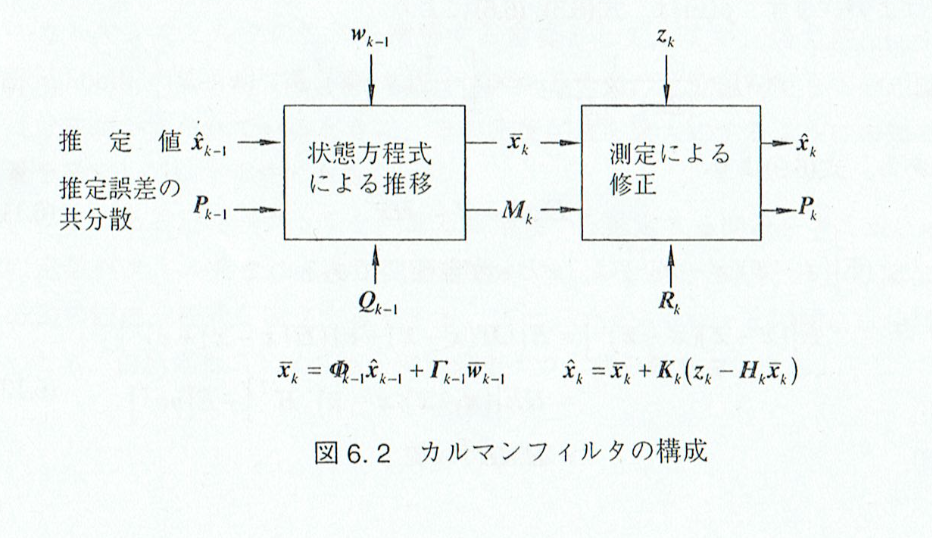
\includegraphics[width=8cm]{../images/kalman_system.png}
    \caption{カルマンフィルタの構成}
    \label{kalman_system}
  \end{center}
  \end{figure}

  \begin{figure}[H]
    \begin{center}
    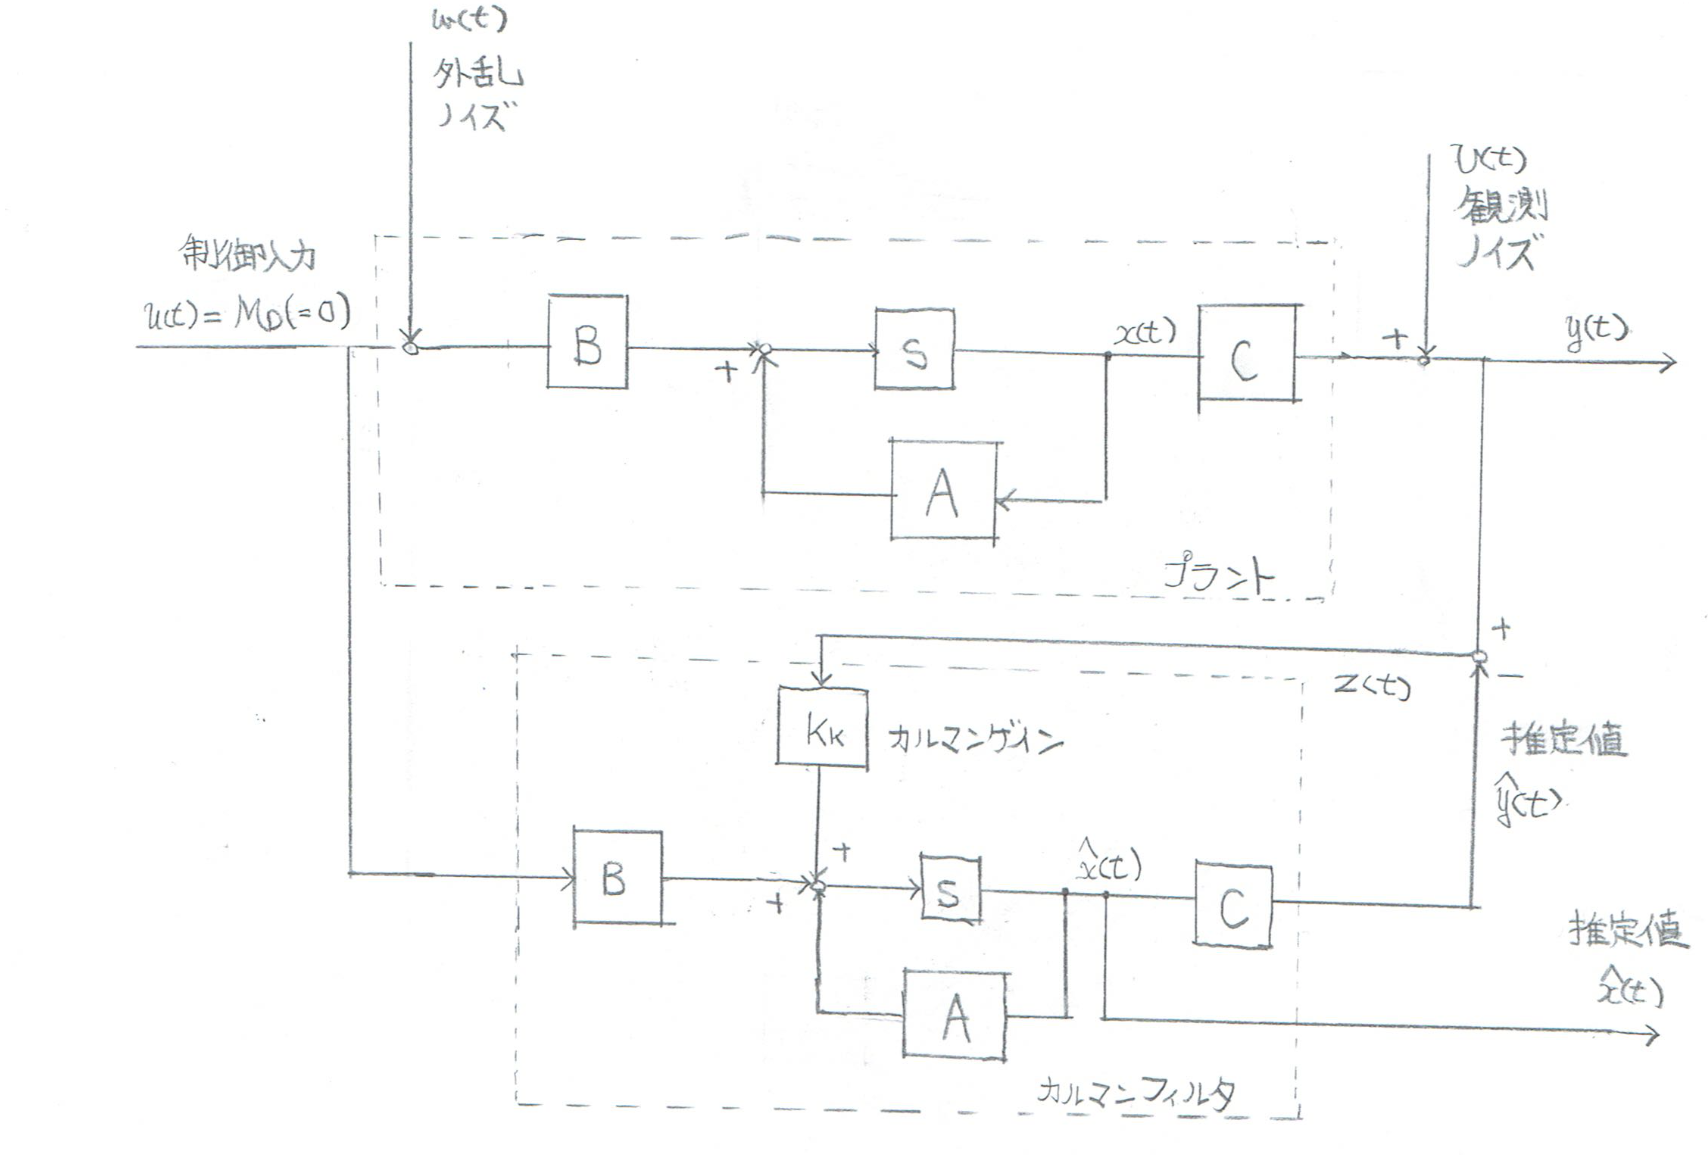
\includegraphics[width=8cm]{../images/kalman_block.png}
    \caption{ブロック線図}
    \label{kalman_block}
  \end{center}
  \end{figure}

\end{enumerate}

\section{結果}
Pの初期条件は,
\begin{equation}
  \bm{P} = \begin{bmatrix}
  \sigma_v & 0 & 0 & 0 & 0 & 0 & 0 \\
  0 & \sigma_v & 0 & 0 & 0 & 0 & 0 \\
  0 & 0 & \sigma_v & 0 & 0 & 0 & 0 \\
  0 & 0 & 0 & \sigma_v & 0 & 0 & 0 \\
  0 & 0 & 0 & 0 & \sigma_w & 0 & 0 \\
  0 & 0 & 0 & 0 & 0 & \sigma_w & 0 \\
  0 & 0 & 0 & 0 & 0 & 0 & \sigma_w
\end{bmatrix}
\end{equation}
とした.結果は以下のようになった.

\begin{figure}[H]
 \begin{minipage}{0.5\hsize}
  \begin{center}
   \includegraphics[width=65mm]{../../../fig/R2qt0v1.png}
  \end{center}
 \end{minipage}
 \begin{minipage}{0.5\hsize}
  \begin{center}
   \includegraphics[width=65mm]{../../../fig/R2qt1v1.png}
  \end{center}
 \end{minipage}
\end{figure}

\vspace{-1cm}

\begin{figure}[H]
 \begin{minipage}{0.5\hsize}
  \begin{center}
   \includegraphics[width=65mm]{../../../fig/R2pmatrix0v1.png}
  \end{center}
  %\caption{qt0}
 \end{minipage}
 \begin{minipage}{0.5\hsize}
  \begin{center}
   \includegraphics[width=65mm]{../../../fig/R2pmatrix0v1.png}
  \end{center}
  %\caption{qt1}
 \end{minipage}
\end{figure}

\begin{figure}[H]
 \begin{minipage}{0.5\hsize}
  \begin{center}
   \includegraphics[width=65mm]{../../../fig/R2qt2v1.png}
  \end{center}
 \end{minipage}
 \begin{minipage}{0.5\hsize}
  \begin{center}
   \includegraphics[width=65mm]{../../../fig/R2qt3v1.png}
  \end{center}
 \end{minipage}
\end{figure}

\vspace{-1cm}

\begin{figure}[H]
 \begin{minipage}{0.5\hsize}
  \begin{center}
   \includegraphics[width=65mm]{../../../fig/R2pmatrix2v1.png}
  \end{center}
  %\caption{qt2}
 \end{minipage}
 \begin{minipage}{0.5\hsize}
  \begin{center}
   \includegraphics[width=65mm]{../../../fig/R2pmatrix3v1.png}
  \end{center}
  %\caption{qt3}
 \end{minipage}
\end{figure}

\vspace{2cm}

\begin{figure}[H]
 \begin{minipage}{0.5\hsize}
  \begin{center}
   \includegraphics[width=65mm]{../../../fig/R2omega1v1.png}
  \end{center}
 \end{minipage}
 \begin{minipage}{0.5\hsize}
  \begin{center}
   \includegraphics[width=65mm]{../../../fig/R2omega2v1.png}
  \end{center}
 \end{minipage}
\end{figure}

\vspace{-1cm}

\begin{figure}[H]
 \begin{minipage}{0.5\hsize}
  \begin{center}
   \includegraphics[width=65mm]{../../../fig/R2pmatrix4v1.png}
  \end{center}
  %\caption{$\omega_x$}
 \end{minipage}
 \begin{minipage}{0.5\hsize}
  \begin{center}
   \includegraphics[width=65mm]{../../../fig/R2pmatrix5v1.png}
  \end{center}
  %\caption{$\omega_y$}
 \end{minipage}
\end{figure}

\begin{figure}[H]
 \begin{minipage}{0.5\hsize}
  \begin{center}
   \includegraphics[width=65mm]{../../../fig/R2omega3v1.png}
  \end{center}
 \end{minipage}
 \begin{minipage}{0.5\hsize}
 \end{minipage}
\end{figure}

\vspace{-1cm}

\begin{figure}[H]
 \begin{minipage}{0.5\hsize}
  \begin{center}
   \includegraphics[width=65mm]{../../../fig/R2pmatrix6v1.png}
  \end{center}
  %\caption{$\omega_z$}
 \end{minipage}
 \begin{minipage}{0.5\hsize}
 \end{minipage}
\end{figure}

推定値が真値に漸近し,また真値とのずれ$\Delta x$も$\sqrt{P_{ii}}$が減少するに従って,
減少していっていることが分かる.

\section{考察}
カルマンフィルターの中核をなすパラメータである, カルマンゲインについて考察する.
カルマンゲイン$\bm{K_k}$は, 第2節でも触れたように観測値とシステム推定値$\bm{\overline{x_k}}$から予測される
観測値との偏差$\bm{(z_k- H_k\overline{x_k})}$を踏まえて,
\begin{equation}
  \hat{x_k} = \overline{x_k} +\bm{K_k(z_k- H_k\overline{x_k})}
\end{equation}
で推定値の更新を行うためのゲインであり,
\begin{equation}
  \bm{K_k} = \bm{P_k H^T R_k^{-1}}
\end{equation}
で与えられる. ここで, $\bm{P_k}$は観測後の推定っs誤差の共分散, $\bm{H^T}$は観測方程式
\begin{equation}
  \bm{z(t)} = \bm{Hx(t)} + \bm{v_k}
\end{equation}
で登場するOutput Matrix, $\bm{R_k}$は測定誤差であった. このカルマンゲインは最尤推定の理論
を用いて数式的に導き出すことができたが, ここではカルマンゲインの定義式自体から,
カルマンゲイン自体が何を指し示しているのか考えてみることにする. \\
定義式を変形していくことを考える.
\begin{align}
  \bm{K_k} &= \bm{P_k H^T R_k^{-1}} \nonumber \\
           &= \bm{{(M_k^{-1}+{H_k}^{T}{R_k}^{-1}H_k)}^{-1}{H_k}^T{R_k}^{-1}}\nonumber \\
           &= \bm{{M_kH_k^{T}}{(R_k + H_kM_k{H_k}^T)}^{-1}}
\end{align}
ここで、$\bm{M_k}$は観測前の推定誤差の共分散である. ここで, わかりやすく極限を考えると
\begin{align}
  \lim_{\bm{R_k} \to 0} \bm{{M_kH_k^{T}}{(R_k + H_kM_k{H_k}^T)}^{-1}} &= {\bm{H_k}}^{-1} \\
  \lim_{\bm{M_k} \to 0} \bm{{M_kH_k^{T}}{(R_k + H_kM_k{H_k}^T)}^{-1}} &= 0 \\
\end{align}
であるから,観測前のシステム推定値の誤差が大きいほどカルマンゲインは小さくなり, 逆に観測ノイズが
小さいほどカルマンゲインは大きくなることが分かる. すなわち,カルマンゲインはどれほど観測値を
システム推定値との比較において信用するかという指標になっていると言える. これを踏まえ, 今回のモデル
において,観測誤差と外乱トルクの誤差の大きさを変化させてカルマンゲインの変化をみるシミュレーションを行った.
まず,最初に提示された初期条件(観測ノイズ$\bm{v}, \sigma_v = 0.01$, 外乱トルク$\bm{w}, \sigma_w = 0.01$)
におけるカルマンゲインの変化は次の図のようになった. フィルターが働き真値に収束していくにつれて,
カルマンゲインのノルムが小さくなっていってることが分かる.

\begin{figure}[H]
  \begin{center}
  \includegraphics[width=8cm]{../../../fig/R2kmatrix1.png}
  \caption{$\bm{v}, \sigma_v = 0.01$,$\bm{w}, \sigma_w = 0.01$の際のカルマンゲインノルム}
\end{center}
\end{figure}

これに対し, $(\sigma_v = 0.02, \sigma_w = 0.02), (\sigma_v = 0.03, \sigma_w = 0.01),
(\sigma_v = 0.01, \sigma_w = 0.03)$としたものについて比較を行ったところ,
以下のようになった.
\begin{figure}[H]
  \begin{center}
  \includegraphics[width=12cm]{../../../fig/R2kmatrix_compare.png}
  \caption{$\sigma_v,\sigma_w$を変化させた際のカルマンゲインノルム}
\end{center}
\end{figure}

観測ノイズ$\bm{v}, \sigma_v$を大きくするとカルマンゲインが小さくなり, 逆に外乱トルク$\bm{w}, \sigma_w$
を大きくするとシステム推定値の誤差が大きくなり, カルマンゲインが大きくなる. \\
またいずれの場合も, 冒頭に非常にカルマンゲインのノルムが大きくなるフェーズがあるが, これは初期誤差($\bm{P}$
の初期値)の関係でシステム推定値の誤差が冒頭大きくなってしまっていることが原因であると考えられる.
これは第3章で並べた$\sqrt{P_{ii}}$の時間履歴において, 冒頭の変化が非常に大きくなっていることからも読み取れる.




\end{document}
